\documentclass{standalone}
\usepackage{tikz}
\usepackage{tikz-feynman} % Paquete para diagramas de Feynman
\begin{document}

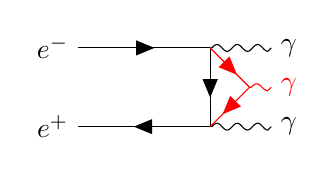
\begin{tikzpicture}
    \begin{feynman}
        % Nodos de partículas
        \vertex (i1) at (-1,1) {\(e^{-}\)};
        \vertex (v1) at (1,1); 
        \vertex (f1) at (2,1) {$\gamma$}; 
        
        \vertex (i2) at (-1,0) {$e^+$}; 
        \vertex (v2) at (1,0); 
        \vertex (f2) at (2,0) {$\gamma$}; 
       
        \vertex (v3) at (1.5,0.5);
        \vertex (f3) at (2,0.5){\textcolor{red}{$\gamma$}};
        % Diagramas de líneas
        \diagram* {
            (i1)--[fermion] (v1)--[boson] (f1),
            (v1)--[fermion] (v2),
            (v2)--[fermion] (i2),
            (v2)--[boson] (f2),

            (v1)--[red,fermion] (v3),
            (v3)--[red,fermion] (v2),
            (v3)--[red,boson] (f3),
        };
    \end{feynman}
\end{tikzpicture}

\end{document}
